\section{Theoretical Analysis}
\label{sec:analysis}

In this section, the circuit shown in \textbf{Figure~\ref{fig:diagram_t4}} is analysed
theoretically.
\begin{figure}[h] \centering
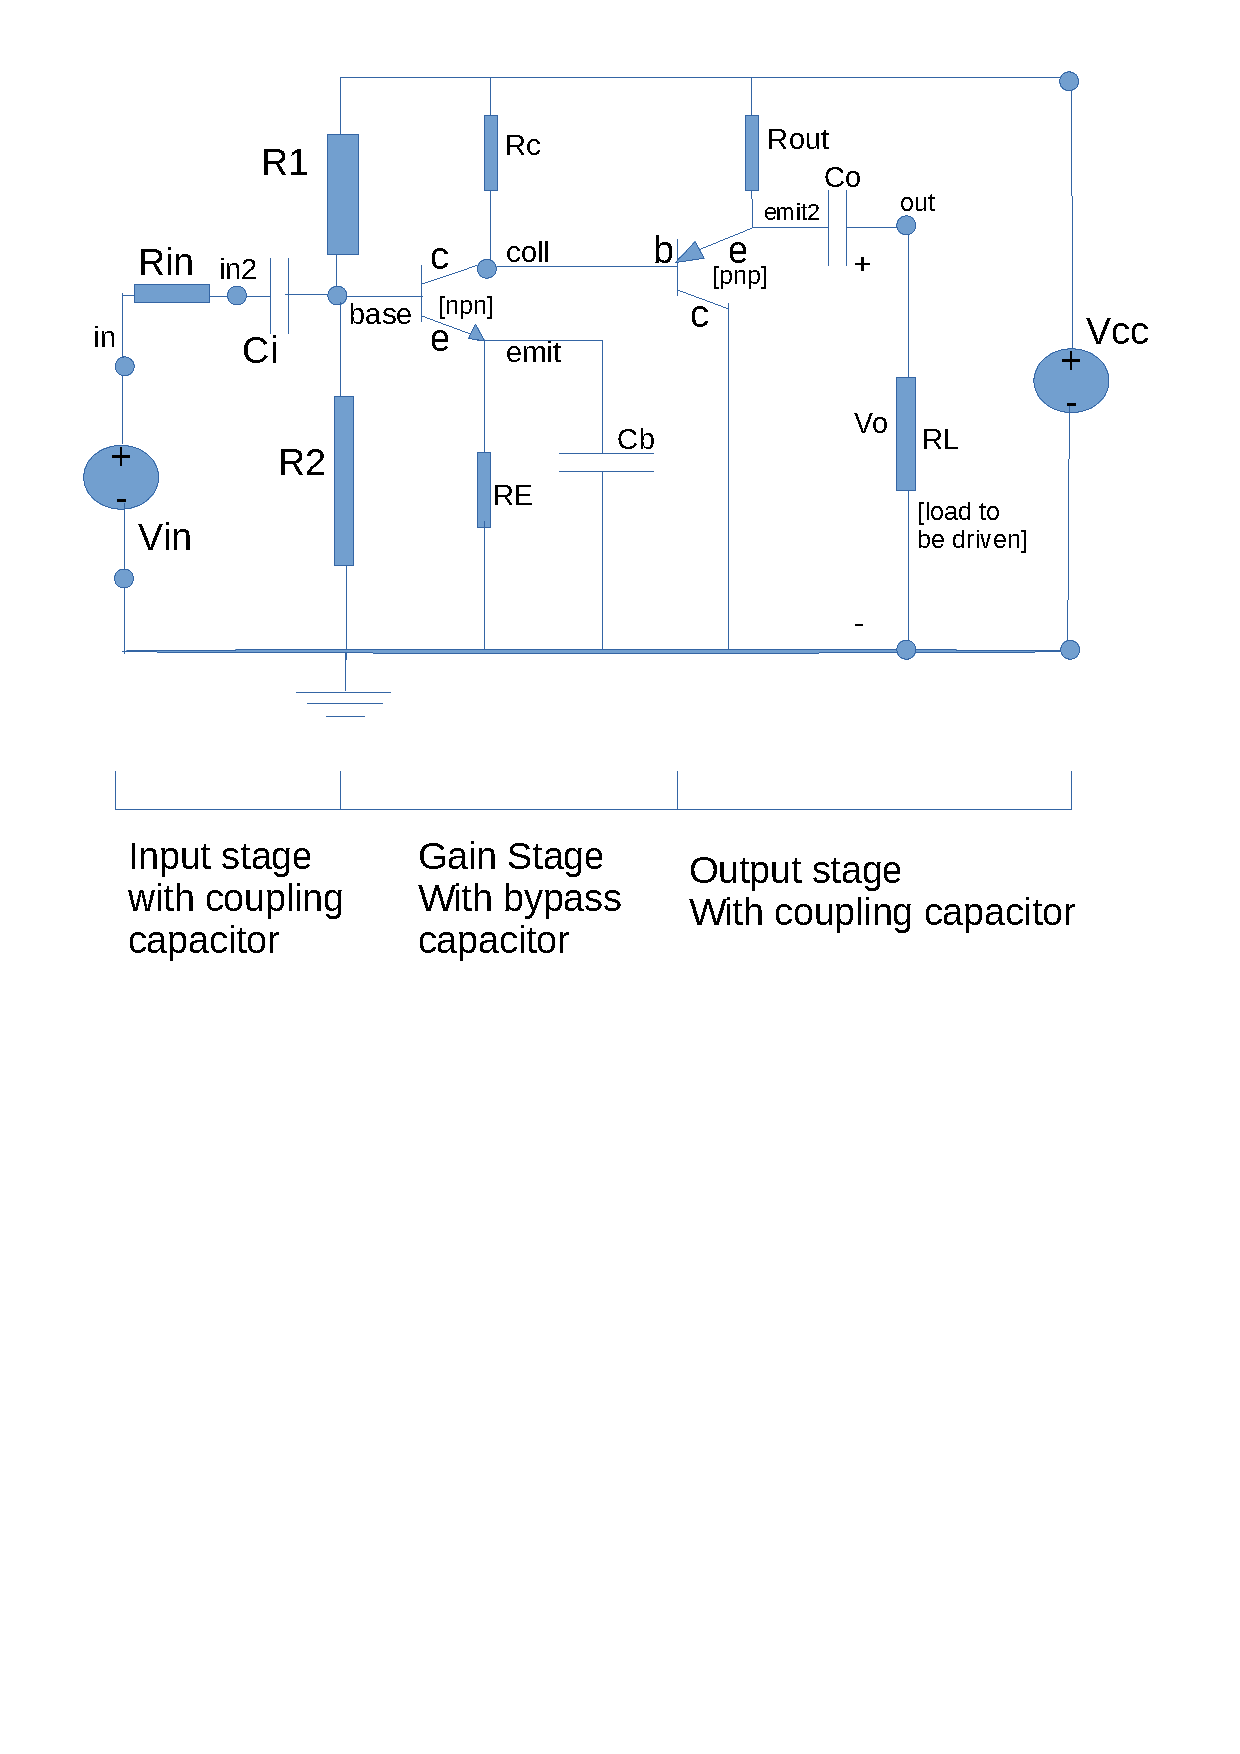
\includegraphics[width=0.95\linewidth]{diagram_t4.pdf}
\vspace{-7cm}
\caption{Diagram of the circuit considered for the computations and simulations.}
\label{fig:diagram_t4}
\end{figure}


As explained before, in the previous section the audio amplifier is composed of two stages.In the first stage (the gain stage) the primary objective is to amplifie the voltage input signal. To do so this section will have an high gain. This stage also has a high input impedance which avoids the degradation of the input signal. The  downside of this stage is its high output impedance that makes it difficult to connect to a speaker without having the signal degrade in the exit. That is why there is an output stage. This stage will have a low output impedance which is very good because it allows us to connect to the speaker without the signal degrading. When we connect the two stages the signal does not degrade beacuse the output stage input impedance is higher than the output impedance of the gain stage, meaning no signal degradation in the transtion between stages. In the output stage the gain is very close to one, meaning than there will be no amplification nor attenuation of the signal.   

The main purpose of the bypass capacitor $C_{E}$ in the gain stage is to avoid a gain loss through resitor ${R_E}$ and the main purpose of resitor ${R_E}$ is to stabilize the temperature effect. In the DC the temperature effect is most important while in AC is the gain. Therefore there needs to be an equilibrium. This components where placed in parallel in order to achive this equilibrium. For lower frequencies (DC) capacitor $C_{E}$ behaves like an open circuit and the current goes through resistor ${R_E}$ stabilizing the temperature effect. For higher frequencies (AC) the capacitor is a short circuit and therefore it is used to bypass the resistor $R_{E}$ avoiding lowering the gain. 


The gain of the audio amplifier, the upper and lower cut off frequency, the bandwidth and the input and output impedances as well as the merit are presented in the following table, both for the theoretical analysis (right) and the Ngspice simulation (left) in order to make a side-by-side comparison.

\hfill
 \parbox{1\linewidth}{
  \centering
  \begin{tabular}{|l|l|l|r|}
    \hline    
    {\bf Parameter} & {\bf Simulation} & {\bf Theoretical } & {\bf Units }\\ \hline
    Zi & 766.402 & 640.49 & Ohm\\ \hline
Zo & 4.49605 & 2.9364 & Ohm\\ \hline
Cost & 8116 & Cost & MU\\ \hline
uco & 3106933.000 & 2123123123123.000 & Hz\\ \hline
lco & 7.924 & 2123123123123.000 & Hz\\ \hline
Bandwidth & 3106925.076 & 2123123123123.000 & Hz\\ \hline
Gainv(out) & 56.041 & -107.220 & [adimensional]\\ \hline
MERIT & 2707.5316 & -104.2260 & gold medals\\ \hline

  \label{tab:results}
  \end{tabular}
  }
  
\vspace{2cm}
    The only difference is in the ripple value, given the Von parameter for the thoeretical model was derived from the simulation results - this accounts for the perfect fit between the simulated and predicted average output voltages. As such, the merit figures differ given the ripple value is found in denominator - this means that, despite the ripple deviation being in the order of microvolts, this deviation is amplified in the merit formula. In adition, the precision of octave and ngspice floating point is different, which may account for part of the differences found. But more importantly, the difference obtained was mainly due to the fact that the models
used for the diodes in the theorethical analysis differ from those used by Ngspice. The diode
model used by Ngspice is way more complex than the one implemented theoretically.
  
  The next figures present the plots required, resulting solely from the theoretical analysis.

%In \textbf{Table~\ref{tab:theoretical}} the values for the branch currents and the node voltages obtained from the Octave script for both methods are presented. Here, the node voltages in the mesh method were computed from the respective currents, which were determined as described in the previous subsection.



\subsection{Output of the voltage regulator circuit, compared with the output sinusoidal voltage of the transformer and the envelope detector voltage}

\par
\begin{figure}[H] \centering
%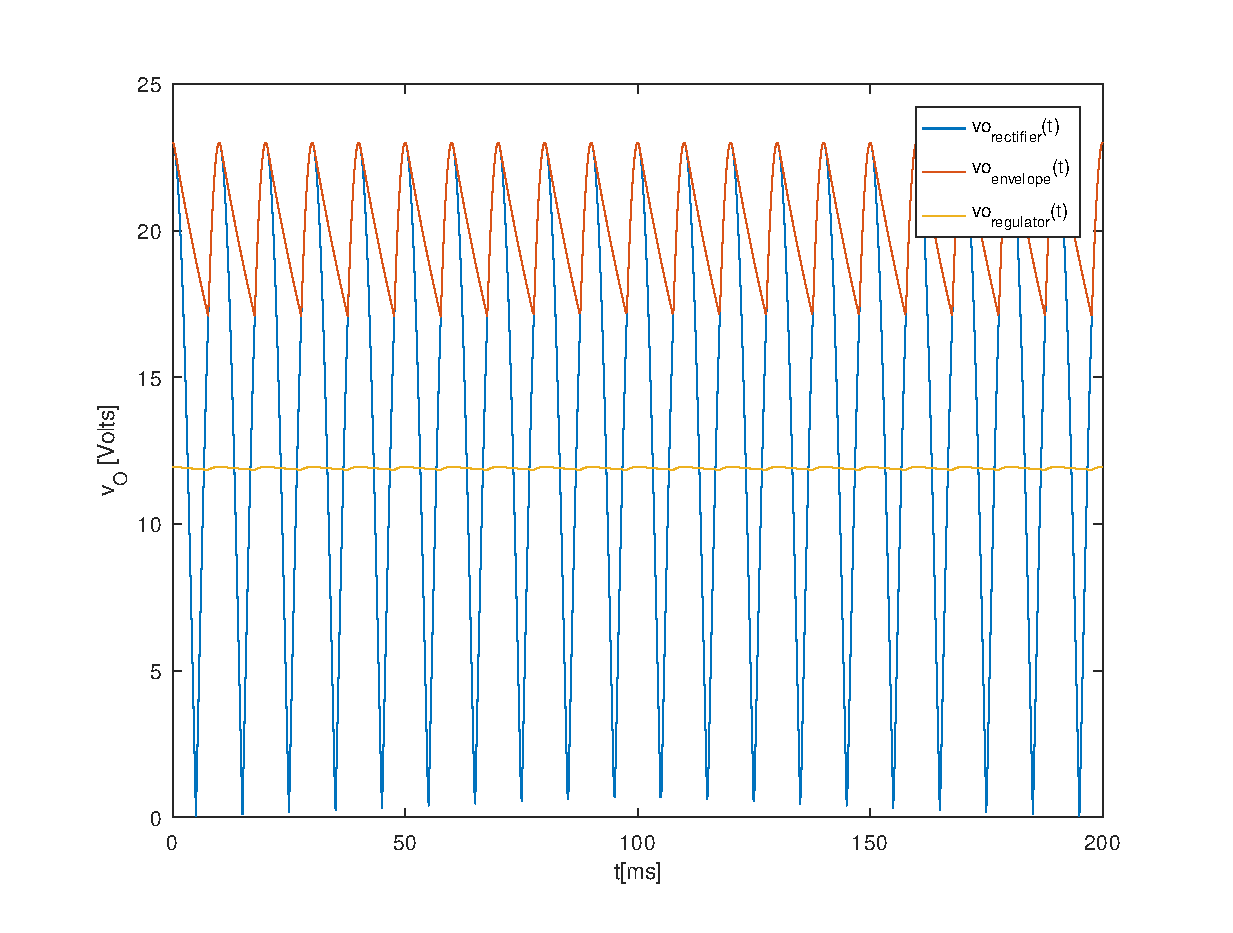
\includegraphics[width=0.6\linewidth]{all_vout.eps}
\caption{Output of the voltage regulator circuit (yellow), compared with the output sinusoidal voltage of the transformer (blue) and the envelope detector voltage (red)}
\label{fig:all_vout}
\end{figure}


\subsection{Output of the Envelope Detector (acting on the output of the full-wave rectifier)}

\par
\begin{figure}[H] \centering
%\includegraphics[width=0.6\linewidth]{envelope.eps}
\caption{Output of the Envelope Detector (acting on the output of the full-wave rectifier)}
\label{fig:envelope}
\end{figure}



\par
\begin{figure}[H] \centering
%\includegraphics[width=0.6\linewidth]{regulator.eps}
\caption{Output of the voltage regulator circuit, so as to visualize the ripple effect in greater detail}
\label{fig:regulator}
\end{figure}

\par
\begin{figure}[H] \centering
%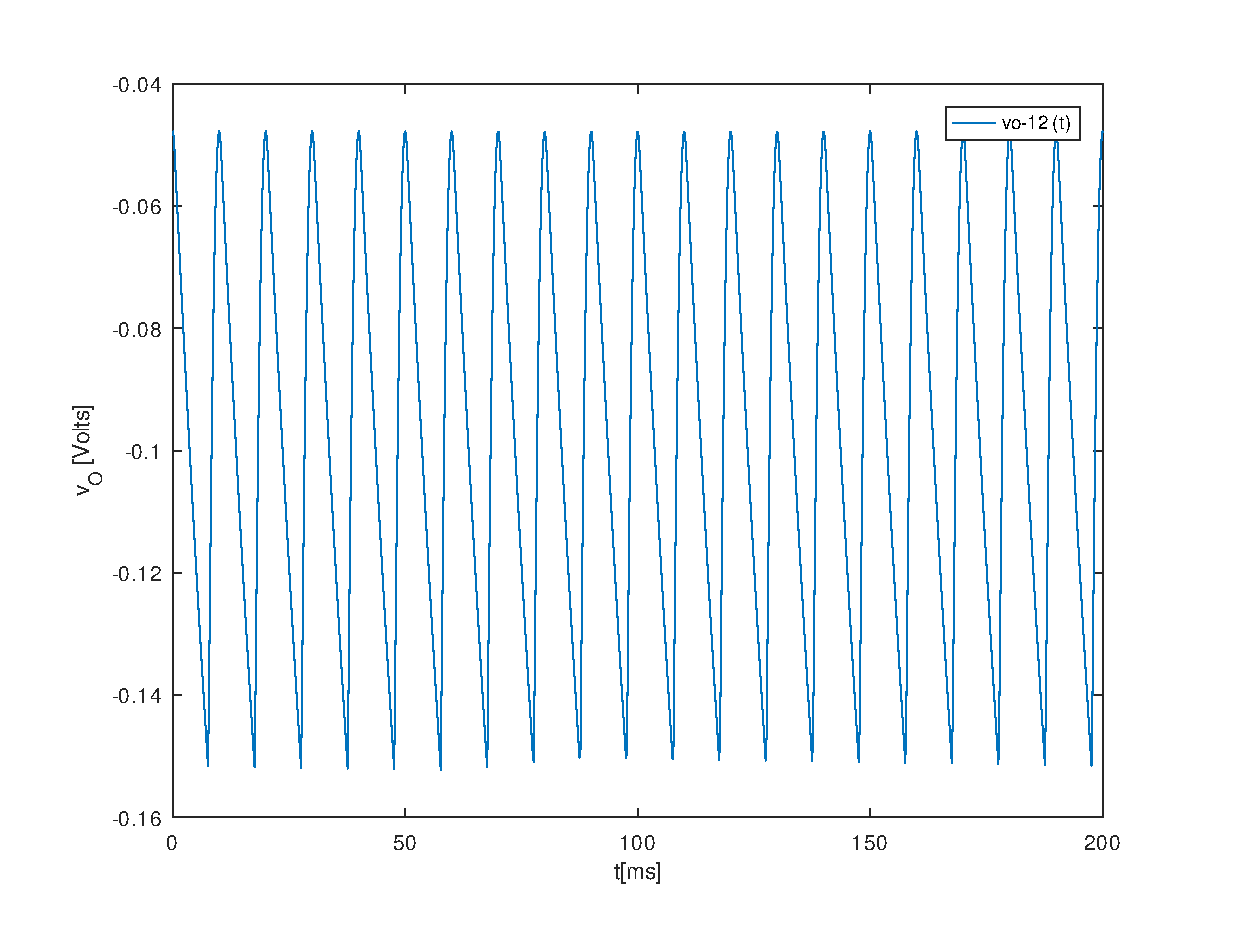
\includegraphics[width=0.6\linewidth]{deviation.eps}
\caption{($v_O$ – 12) (output AC component + DC deviation)}
\label{fig:deviation}
\end{figure}


%\begin{figure}[H] \centering
%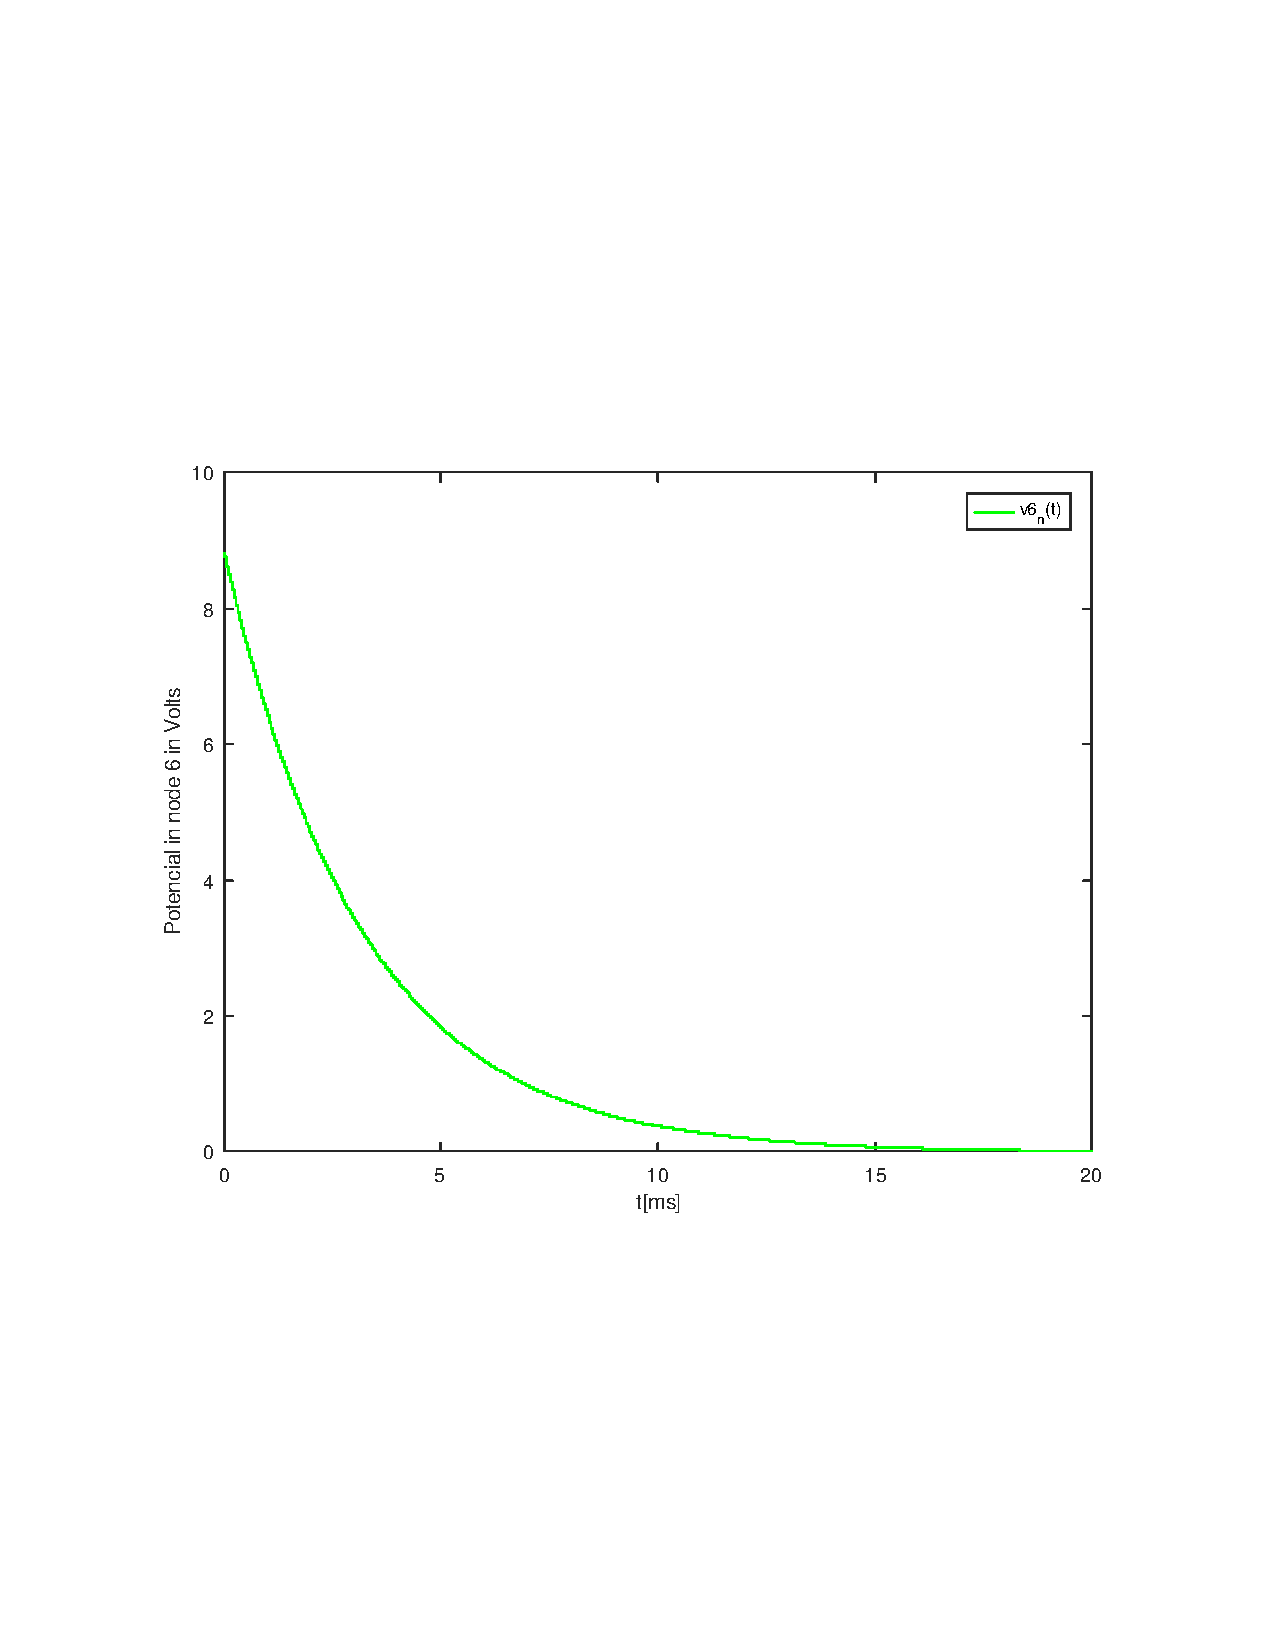
\includegraphics[width=0.9\linewidth]{natural_tab.pdf}
%\caption{Natural response of $V_6$ as a function os time in the interval from [0,20] ms}
%\label{fig:natural}
%\end{figure} 



%\begin{figure}[H] \centering
%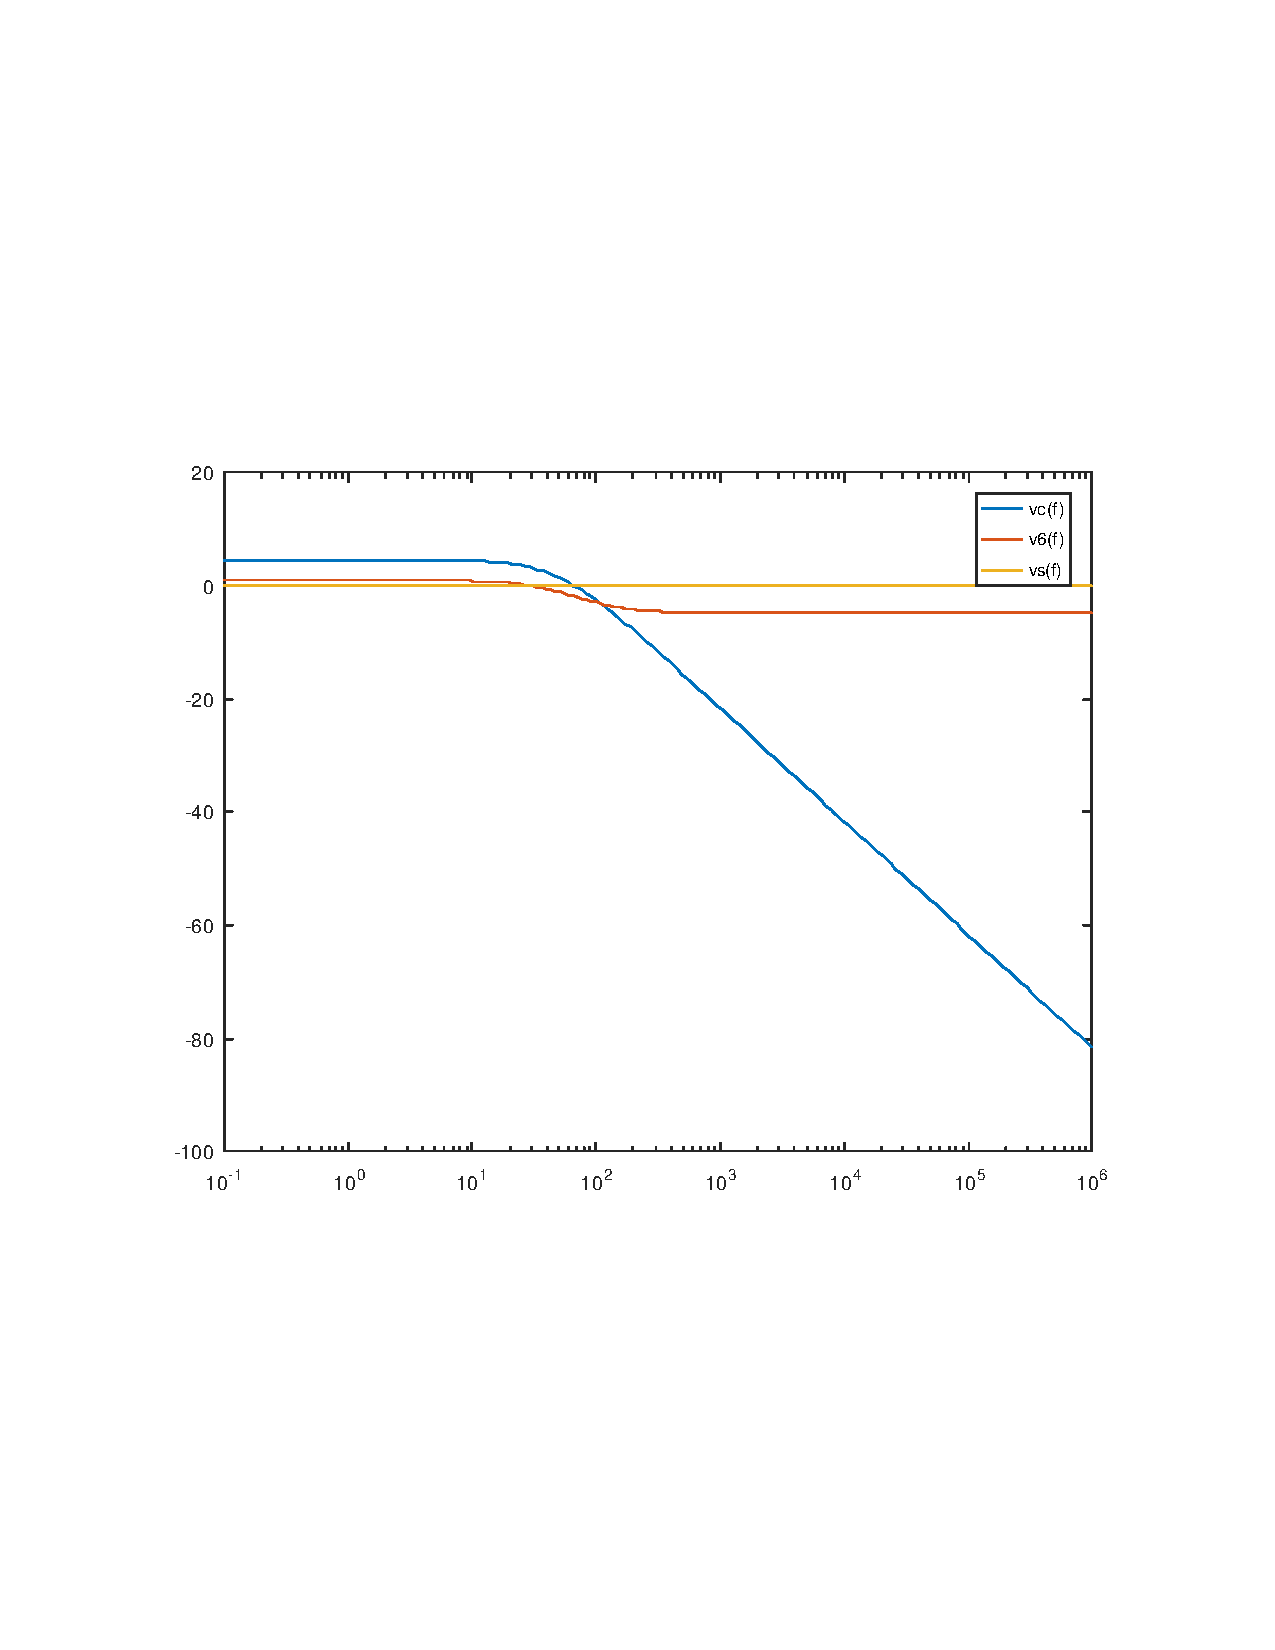
\includegraphics[width=0.9\linewidth]{freq_resp_tab.pdf}
%\caption{Graph for amplitude frequency response, in dB, of $V_c$, $V_6$ and $V_s$ for frequencies ranging from 0.1Hz to 1MHz (logarithmic scale).}
%\label{fig:freq_resp}
%\end{figure}




\pagebreak


